\section{Preliminaries}
\label{sec:preliminaries}
% Definitions and notation used throughout the paper, known results with citations.
% Guidance: knowledge/writing/paper-structure.md, knowledge/writing/math-writing.md

Preliminaries text.

% --- Example (remove): definition, figure, table --------------------------------------------
% Labels: prefix + lowercase words with hyphens; \label directly after \caption.

\begin{definition}[Cut-path]
\label{def:cut-path}
Let $G = (V, E)$ be a graph and $u, v \in V$.
A set $S \subseteq E$ is a \emph{cut-path} if \dots
\end{definition}

\begin{figure}[tb]
  \centering
  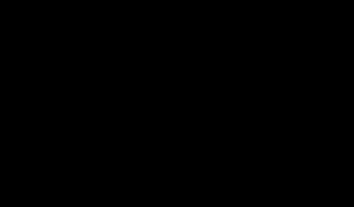
\includegraphics[width=0.6\linewidth]{img/example}   % vector PDF; file name lowercase-with-hyphens
  \caption{What the reader should see, in one sentence.}
  \label{fig:example}
\end{figure}

\begin{table}[tb]
  \centering
  \caption{Caption above the table. Running time in seconds, mean of 10 runs.}
  \label{tab:runtime}
  \begin{tabular}{@{}lrr@{}}
    \toprule
    Instance & $\abs{V}$ & Time (s) \\
    \midrule
    \texttt{grid-10} & 100 & 0.12 \\
    \texttt{grid-20} & 400 & 1.85 \\
    \bottomrule
  \end{tabular}
\end{table}

\Cref{fig:example} shows \dots; \cref{tab:runtime} lists \dots
